We demonstrate the data movement performance of our OPTIQ framework and existing MPI routines on three communication patterns -- {\em disjoint}, {\em overlap} and {\em subset}, illustrated in Figure \ref{fig:patterns}. In this figure, m and n refer to set of source or destination nodes. These patterns are owing to different possible relationships between source and destination nodes as described below:
\begin{itemize}
\item Disjoint: There are distinct sources and destinations. It is a common data movement pattern present in many applications.
\item Overlap: The sources and destinations are overlapped sets. Some applications like CESM uses this communication pattern for coupling.
\item Subset: Either the set of source nodes is subset of the destination nodes or vice versa. This pattern can be found in CESM and in collective I/O aggregation phase.
\end{itemize}
\begin{figure}[ht]
\vspace{-0.15in}
\centering
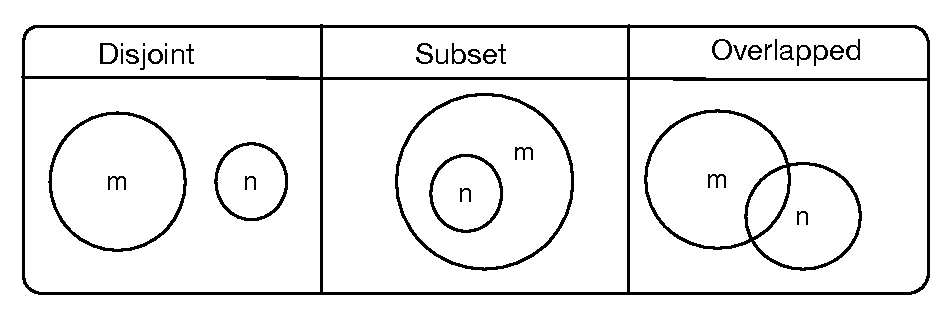
\includegraphics[scale=0.48]{figures/patterns.pdf}
\vspace{-0.15in}
\caption{\small Communication patterns}
\vspace{-0.15in}
\label{fig:patterns}
\end{figure}

We demonstrate throughput improvement in a complex network like 5D torus through the above diverse communication patterns. We compare the efficacy of our algorithms with MPI\_Alltoallv, which is the most commonly used MPI collective for the data movement patterns considered in our work.
